\chapter{Конструкторская часть}

\section{Схемы алгоритмов}

На рисунке~\ref{images:Zbuffer} представлена схема алгоритма Z-буфера.

\begin{figure}[H]
    \centering
    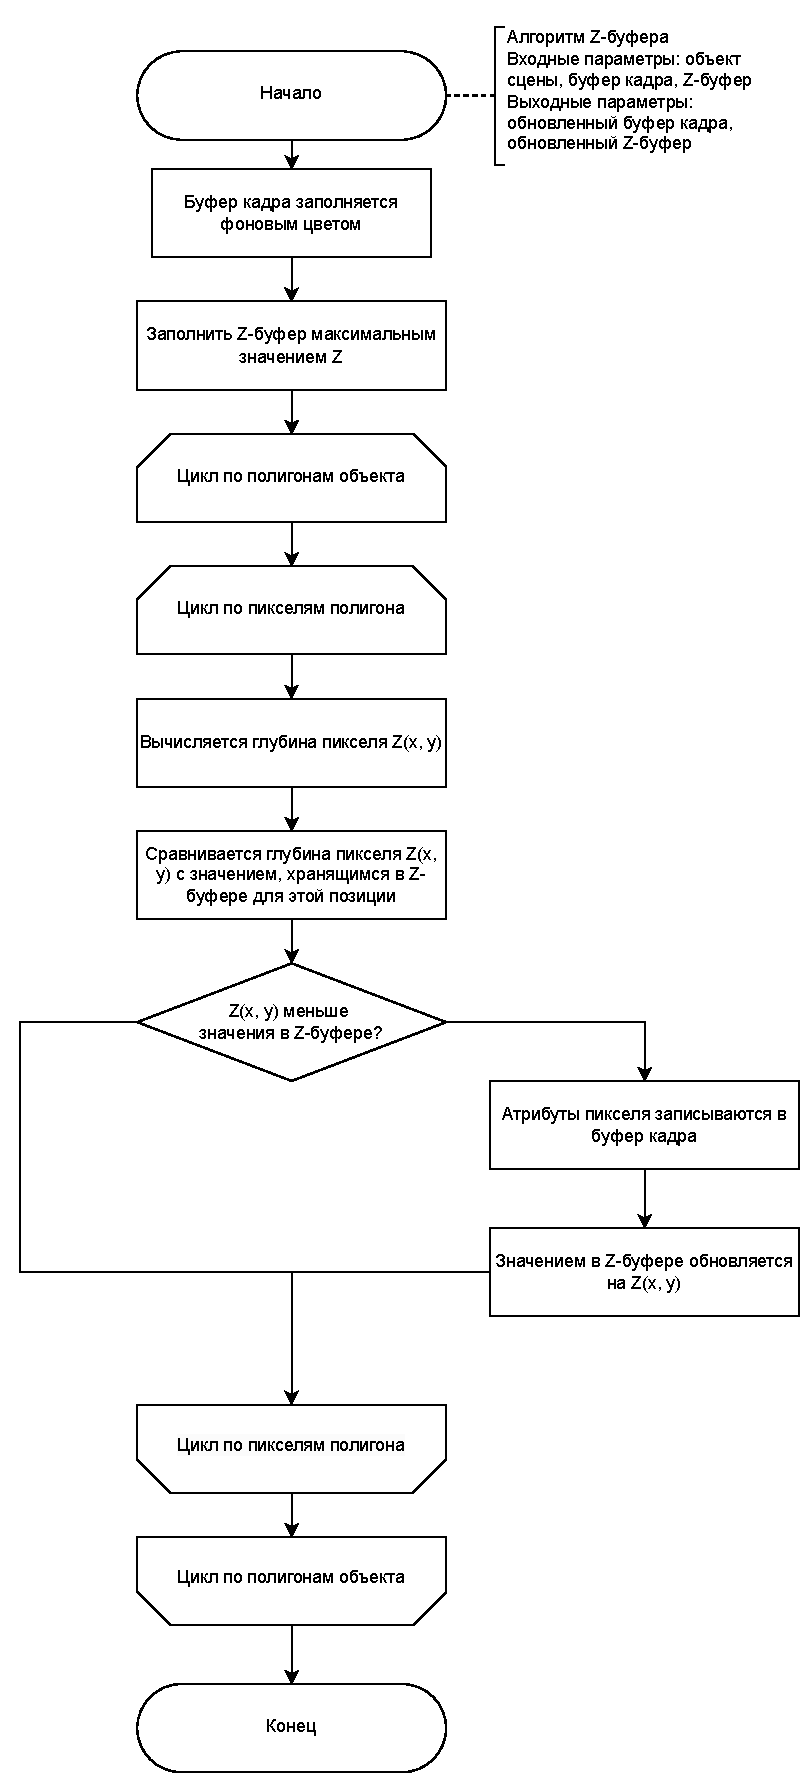
\includegraphics[width=93mm]{images/Zbuffer}
    \caption{Схема алгоритма Z-буфера.}
    \label{images:Zbuffer}
\end{figure}

\vspace{2cm}
На рисунках~\ref{images:Wind_1},~\ref{images:Wind_2} представлена схема алгоритма реализации ветра.

\begin{figure}[H]
    \centering
    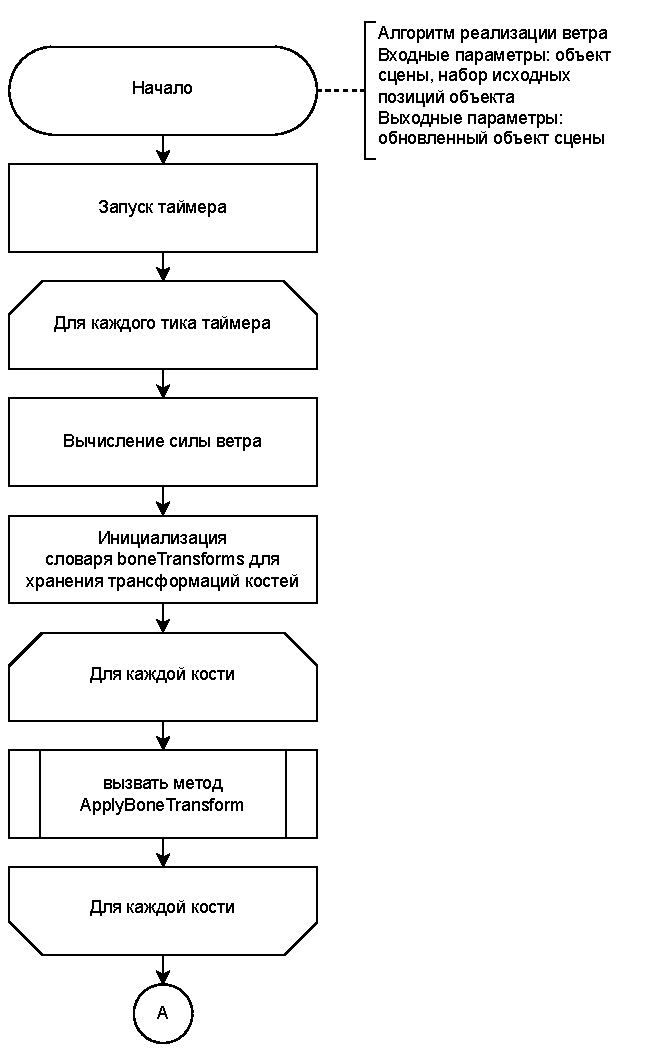
\includegraphics[width=115mm]{images/Wind_1}
    \caption{Схема алгоритма реализации ветра. Часть 1.}
    \label{images:Wind_1}
\end{figure}

\begin{figure}[H]
    \centering
    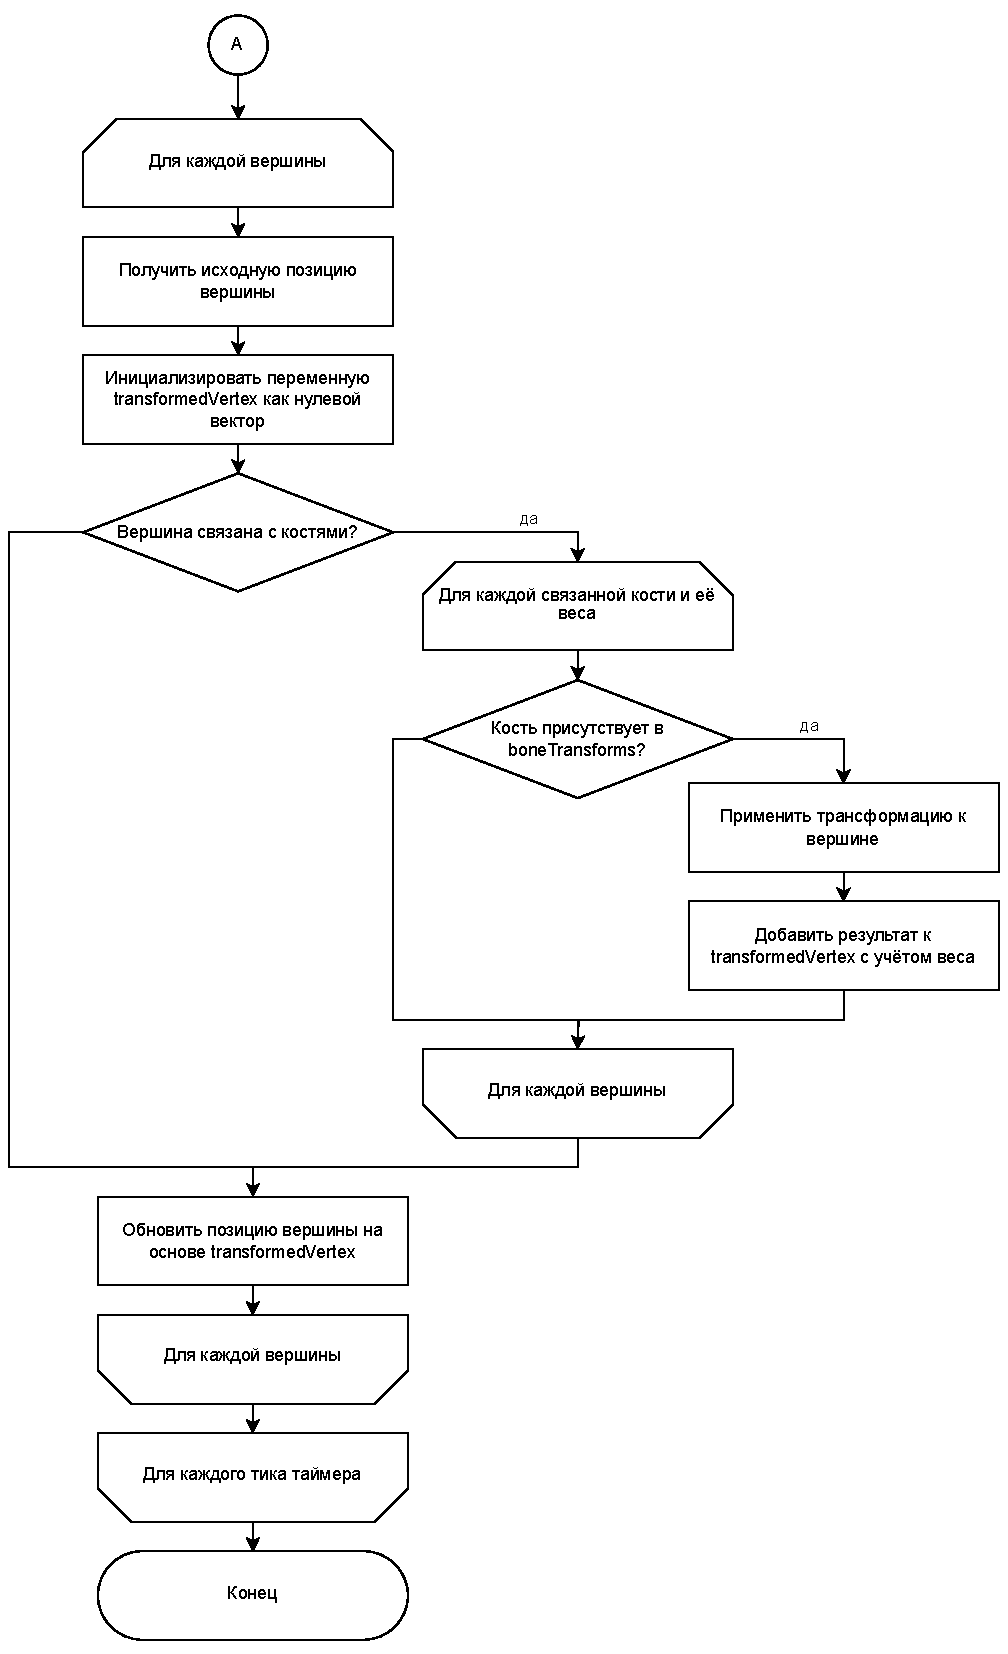
\includegraphics[width=115mm]{images/Wind_2}
    \caption{Схема алгоритма реализации ветра. Часть 2.}
    \label{images:Wind_2}
\end{figure}


На рисунке~\ref{images:ApplyBoneTransform} представлен метод для применения вращения к вершинам кости.
\begin{figure}[H]
    \centering
    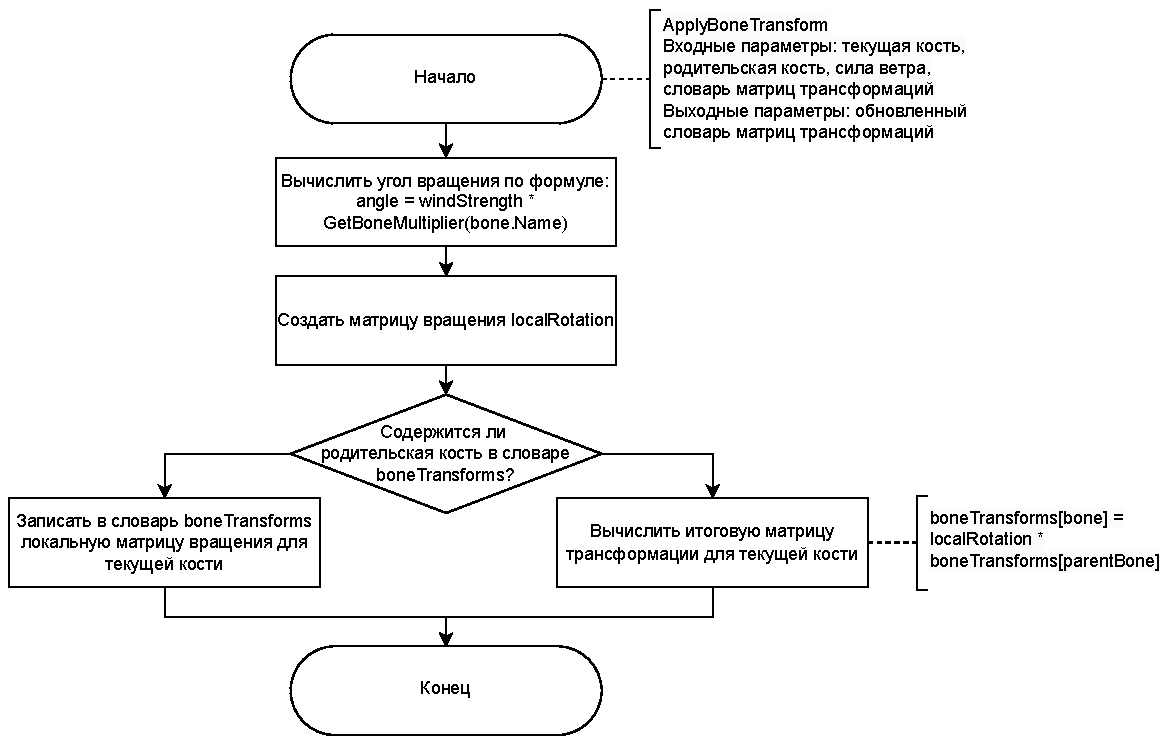
\includegraphics[width=135mm]{images/ApplyBoneTransform}
    \caption{Метод для применения вращения к вершинам кости.}
    \label{images:ApplyBoneTransform}
\end{figure}


\vspace{2cm}
На рисунке~\ref{images:Raycasting} представлена схема алгоритма рендеринга методом Raycasting.

\begin{figure}[H]
    \centering
    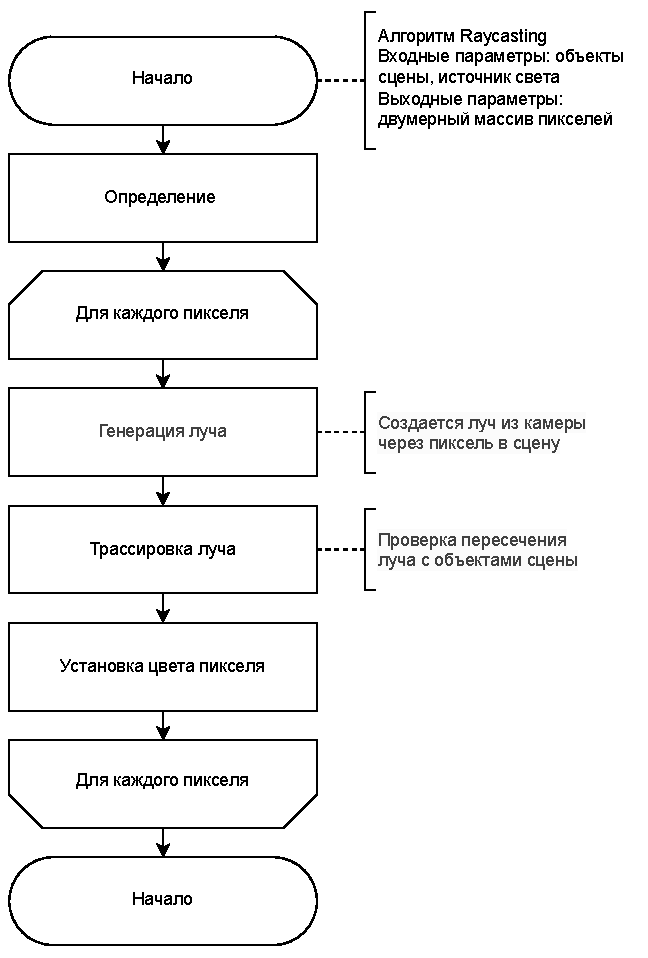
\includegraphics[width=110mm]{images/Raycasting}
    \caption{Схема алгоритма рендеринга методом Raycasting.}
    \label{images:Raycasting}
\end{figure}

\section{Вывод}

В данном разделе были представлены схемы используемых алгоритмов.